\documentclass[unknownkeysallowed, 10pt, a4 paper, handout]{beamer}

% Custom beamer theme
\usepackage{../style/beamerthemeCustom}
\newcommand{\HRule}{\rule{\linewidth}{0.5mm}}   %FOR TITLEPAGE

\usepackage{changepage}       % adjustwidth

\setlength\parskip{0.3cm}

\newcommand{\focus}[1]{\textbf{\textcolor{red}{#1}}}
\newcommand{\ra}{$\longrightarrow$ }
\newcommand{\lra}{$\longleftrightarrow$ }

\newcommand{\code}[1]{\colorbox{black}{\color{green}\texttt{#1}}}

% Command to create two side-by-side minipages
\newcommand{\sidebyside}[5]{
  \begin{minipage}{#1\textwidth}
    #2
  \end{minipage} #3 \begin{minipage}{#4\textwidth}
    #5
  \end{minipage}
}

\begin{document}


\begin{frame}[label=outline]{Science with the Computer}
  You can do Science with a computer !
  \begin{columns}[T]
    \begin{column}{.53\textwidth}
      \begin{itemize}
        \item Text Editors and WYSIWYG programs for writing
        \item Tools and libraries for data handling and visualization
        \item Data acquisition and storage
        \item Modelling and numerical algorithms
      \end{itemize}
    \end{column}
    \hfill
    \begin{column}{.45\textwidth}
      \vspace{15pt}
      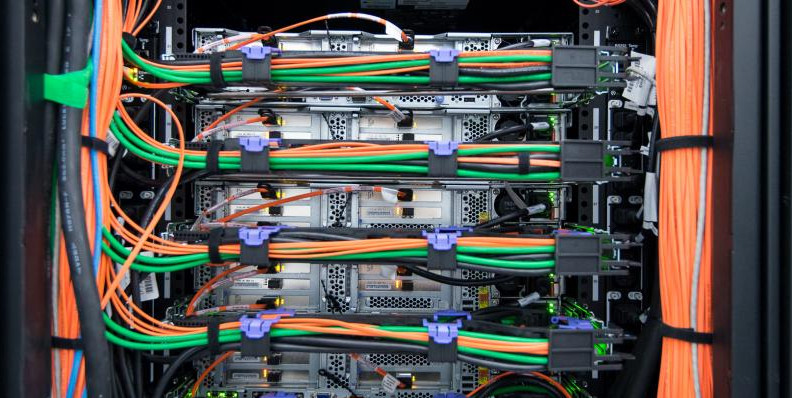
\includegraphics[scale=0.2]{pics/20140924103021_DSC_6759_MHPC.jpg}
    \end{column}
  \end{columns}
  It can get to such complexities that a whole new Science has emerged:
  \begin{center}
    \textcolor{red}{Computer Science} : 
             study of computers and computational systems
  \end{center}
\end{frame}


\begin{frame}[label=textedit]{Text editing}
  \begin{center}
  Pick your choice !
  \end{center}
  \begin{columns}[T]
    \begin{column}{.55\textwidth}
      \begin{itemize}
        \item Local file: every desktop environment has a text editor
        \begin{itemize}
          \item GNOME : gedit, geany
          \item KDE (Plasma) : kwrite
          \item Xfce : mousepad \\
            \dots
        \end{itemize}
        \item Text console: religious wars !
        \begin{itemize}
          \item vi(m) : Unix pure and true !
          \item emacs : I love GNU !
          \item nano  : I hate both of the above \\
            \dots
        \end{itemize}
      \end{itemize}
    \end{column}
    \hfill
    \begin{column}{.45\textwidth}
      \vspace{10pt}
       
\includegraphics[scale=0.1]{pics/manuscript.jpg}
    \end{column}
  \end{columns}
\end{frame}


\begin{frame}[label=vim1]{Unix vi - 1}
  Starts by: \code{vim filetoedit.ext}
  \begin{columns}[T]
    \begin{column}{.83\textwidth}
      \begin{itemize}
        \item Modes
        \begin{itemize}
           \item \textbf{command mode}: Editor starts in command mode.
              Cursor movement, text deletion, pasting is possible.
              Can close/open files, save and quit editor.
           \item \textbf{insertion mode}: Begins upon entering an insertion
              or change command.
        \end{itemize}
        \item The [ESC] key returns the editor to command mode.
        \item Commands are executed by pressing the return key.
        \item To quit:
        \begin{itemize}
           \item Saving the file: \code{:x}
           \item Without saving the file: \code{:q!}
        \end{itemize}
      \end{itemize}
    \end{column}
    \hfill
    \begin{column}{.25\textwidth}
      
\includegraphics[scale=0.08]{pics/vim.png}
    \end{column}
  \end{columns}
\end{frame}


\begin{frame}[label=vim2]{Unix vi - 2}
  \begin{columns}[T]
    \begin{column}{.83\textwidth}
      \begin{itemize}
        \item To enter insert mode:
        \begin{itemize}
           \item \code{i} insert in the current position
           \item \code{I} insert at line beginning
           \item \code{a} append after character
           \item \code{A} append at end of the line
           \item \code{r} overwrite one character
           \item \code{R} enter replace mode
           \item \code{o} new line inserted below
           \item \code{O} new line inserted above
        \end{itemize}
        \item Move around in command mode:
        \begin{itemize}
          \item \code{h,j,k,l} or arrows in insert mode: left-down-up-right
          \item \code{w,e,b} next/previous word beginning or end
          \item \code{(,)} next/previous sentence 
          \item \code{\{,\}} next/previous paragraph 
          \item \code{0,\$} beginning/end of line
          \item \code{gg,G} beginning/end of file
        \end{itemize}
      \end{itemize}
    \end{column}
    \hfill
    \begin{column}{.25\textwidth}
      
\includegraphics[scale=0.08]{pics/vim.png}
    \end{column}
  \end{columns}
\end{frame}


\begin{frame}[label=vim3]{Unix vi - 3}
  \begin{columns}[T]
    \begin{column}{.83\textwidth}
      \begin{itemize}
        \item change text
        \begin{itemize}
          \item \code{C} change to the end of line
          \item \code{Ncw} change N words
        \end{itemize}
        \item Delete text
        \begin{itemize}
           \item \code{xX} delete character to right/left
           \item \code{D} delete to the end of the line
           \item \code{dd,:d} delete the whole line
           \item \code{Ndd} delete N lines
           \item \code{Ndw} delete N words
        \end{itemize}
        \item Copy text
        \begin{itemize}
          \item \code{yy,:y} copy the line
          \item \code{Nyy} copy N lines
        \end{itemize}
        \item Paste text
        \begin{itemize}
          \item \code{pP} paste the line(s) after/before current
        \end{itemize}
      \end{itemize}
    \end{column}
    \hfill
    \begin{column}{.25\textwidth}
      
\includegraphics[scale=0.08]{pics/vim.png}
    \end{column}
  \end{columns}
\end{frame}


\begin{frame}[label=vim4]{Unix vi - 4}
  \begin{columns}[T]
    \begin{column}{.83\textwidth}
      \begin{itemize}
        \item Search
        \begin{itemize}
          \item \code{/string} Search string ahead
          \item \code{?string} Search string backward
          \item \code{n,N} Next item ahead/backward
        \end{itemize}
        \item Substitute
        \begin{itemize}
           \item \code{:s/pattern/string/} substitute pattern with string
           \item \code{:s!/path/subst!/new/path/!} for a file path
           \item \code{:s/pattern/string/g} all occurences in line
           \item \code{:M,N s/pattern/string/g} all in lines M to N
           \item \code{:1,\$ s/pattern/string/g} all occurences in file
        \end{itemize}
        \item Undo, redo, join, capitalize
        \begin{itemize}
          \item \code{.} Repeat last change
          \item \code{u,U} undo the last/all changes in line
          \item \code{Ctrl+r} Redo the change
          \item \code{J} Join with next line
          \item \code{\~} change case
        \end{itemize}
      \end{itemize}
    \end{column}
    \hfill
    \begin{column}{.25\textwidth}
      
\includegraphics[scale=0.08]{pics/vim.png}
    \end{column}
  \end{columns}
\end{frame}


\begin{frame}[label=pipelining]{Writing your own program - 1}
  Use the building blocs of existing programs and create a complex
  \textcolor{red}{\textbf{pipeline}} of stages to reach the desired processing
  \begin{columns}[T]
    \begin{column}{.33\textwidth}
      \vspace{20pt}
      
\includegraphics[scale=0.25]{pics/plumbing-pipes.png}
    \end{column}
    \hfill
    \begin{column}{.66\textwidth}
      \begin{itemize}
        \item \textbf{Pros} : No programming in the general sense involved,
          just carefully examination of the input and output of existing
          system programs to create the required processing. The REAL UNIX way
          of using a computer.
        \item \textbf{Cons} : Limited by the possible processing allowed by
          system programs, generally related to text file manipulation,
          non portable across different systems
      \end{itemize}
    \end{column}
  \end{columns}
  Example:
  \begin{center}
    \code{ls -al | grep \${USER} | tr -s ' ' | cut -d " " -f 5 > sizes.txt}
  \end{center}
\end{frame}


\begin{frame}[label=scripting]{Writing your own program - 2}
  Use generic \textcolor{red}{\textbf{scripting language}} interpreters which
  can more flexibly allow runtime evaluation of a processing
  \begin{columns}[T]
    \begin{column}{.66\textwidth}
      \begin{itemize}
        \item \textbf{Pros} : More flexible, eventually the shell itself can be
          used, can use specialized libraries for compute intensive tasks,
          rapid prototyping
        \item \textbf{Cons} : Need to learn a programming language, not as
          fast as a system binary can be.
      \end{itemize}
    \end{column}
    \hfill
    \begin{column}{.33\textwidth}
      \vspace{10pt}
      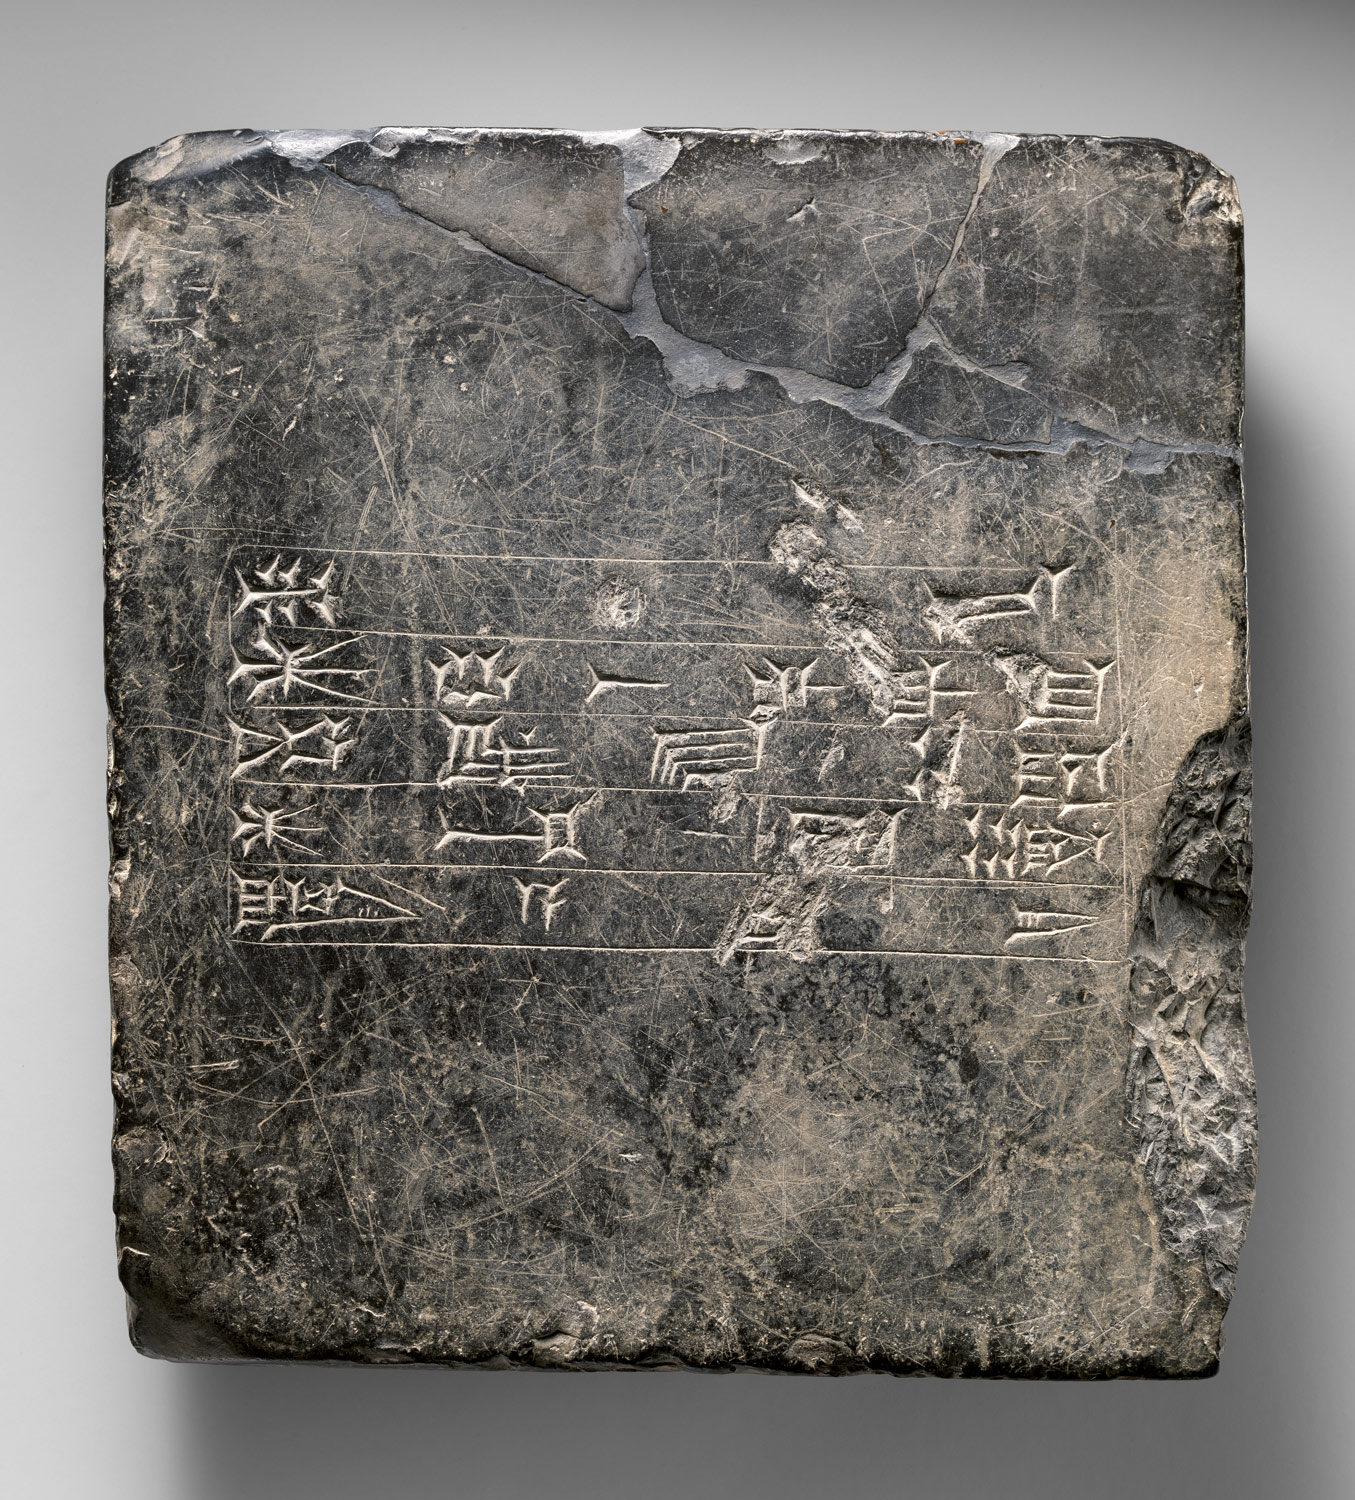
\includegraphics[scale=0.07]{pics/cuneiform.jpg}
    \end{column}
  \end{columns}
  Example:
  \begin{itemize}
    \item Shell scripting
    \item Python language
    \item R statistical language
  \end{itemize}
\end{frame}


\begin{frame}[label=compiled]{Writing your own program - 2}
  Use a low level \textcolor{red}{\textbf{programming language}} which is
  parsed by a program called \textit{compiler} to create a system binary
  program
  \begin{columns}[T]
    \begin{column}{.23\textwidth}
      
\includegraphics[scale=0.35]{pics/225px-ISO_C++_Logo.png}
    \end{column}
    \hfill
    \begin{column}{.76\textwidth}
      \begin{itemize}
        \item \textbf{Pros} : Fast execution time, tailored processing to the
          problem to solve
        \item \textbf{Cons} : Need to learn a programming language, not as
          flexible as a scripting language, may require writing code even
          for very simple and common tasks best approached by generic 
          system programs.
      \end{itemize}
    \end{column}
  \end{columns}
  Example:
  \begin{itemize}
    \item Fortran Programming Language
    \item C/C++ Programming Language
  \end{itemize}
\end{frame}


\begin{frame}[label=Fortran]{Fortran program}
  \begin{center}
  \Large{Fortran source files are text files}
  \end{center}
  \begin{columns}[T]
    \begin{column}{.23\textwidth}
      \vspace{30pt}
      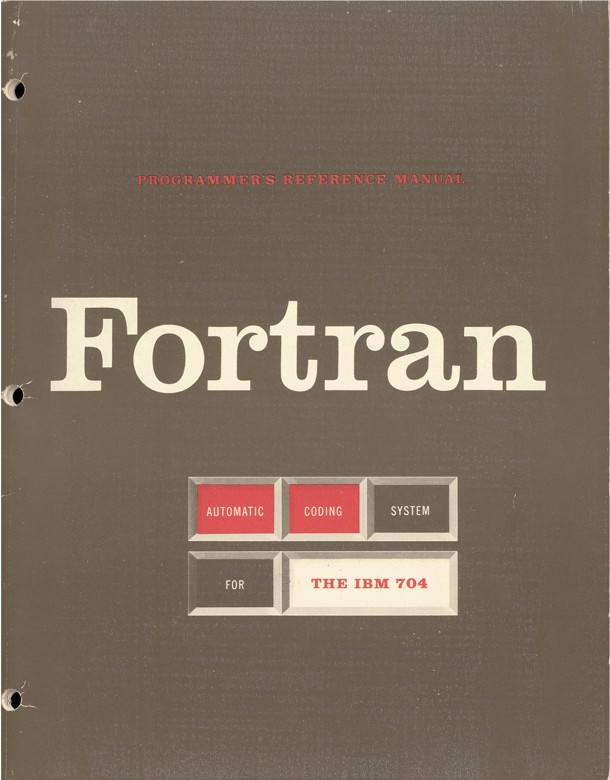
\includegraphics[scale=0.15]{pics/Fortran_acs_cover.jpeg}
    \end{column}
    \hfill
    \begin{column}{.76\textwidth}
      \begin{itemize}
        \item \normalsize{The User writes the source file:} \\
          \footnotesize{
          \code{program myprog} \\
          \code{  print *, 'Hello world'} \\
          \code{end program myprog}
          }
        \item \normalsize{A compiler parses source files and create
           binary object files:} \\
          \footnotesize{
          \code{gfortran -o myprog myprog.f90}
          }
        \item \normalsize{Objects are linked with other objects or
           libraries to create executables:} \\
          \footnotesize{
          \code{0000000 457f 464c 0102 0001 0000 0000 0000 0000} \\
          \code{0000010 0003 003e 0001 0000 06f0 0000 0000 0000} \\
          \code{0000020 0040 0000 0000 0000 1a78 0000 0000 0000} \\
          \code{0000030 0000 0000 0040 0038 0009 0040 001d 001c} \\
          \code{0000040 0006 0000 0004 0000 0040 0000 0000 0000}
          }
      \end{itemize}
    \end{column}
  \end{columns}
\end{frame}


\begin{frame}[label=compiler]{Compiler flags}
  The compiler is a program and accepts command line arguments
  \begin{itemize}
    \item \code{-g}
    \begin{itemize}
      \item include debugging information
    \end{itemize}
    \item \code{-Wall}
    \begin{itemize}
      \item Enables commonly used warning options pertaining to usage
        recommend avoiding and that are easy to avoid
    \end{itemize}
    \item \code{-pedantic}
    \begin{itemize}
      \item check program for Fortran 95 standard conformance
    \end{itemize}
    \item \code{-fbacktrace}
    \begin{itemize}
      \item print the whole trace of the error
    \end{itemize}
    \item \code{-fcheck=all}
    \begin{itemize}
      \item perform all available run-time checks
    \end{itemize}
    \item \code{-Ofast}
    \begin{itemize}
      \item Optimize for fast execution time
    \end{itemize}
  \end{itemize}
\end{frame}


\begin{frame}[label=makefile]{Make program}
  The traditional way to manage a project code is the \code{make} program
  \begin{columns}[T]
    \begin{column}{.23\textwidth}
      \vspace{30pt}
      
\includegraphics[scale=0.25]{pics/GM.jpg}
    \end{column}
    \hfill
    \begin{column}{.76\textwidth}
      \begin{itemize}
        \item \code{[Mm]akefile}
        \begin{itemize}
          \item For each directory in a project, you provide a Makefile.
          \item The makefile contains:
          \begin{itemize}
             \item \textbf{Targets} : things you can ask to be made
             \item \textbf{Dependencies} : order of things to be made
             \item \textbf{Variables} : useful to store options
             \item \textbf{Conditionals} : select how to do on variable value
          \end{itemize}
          \item A hyerarchy of Makefiles can be built
          \item For very complex projects Makefiles can be generated through
             other tools
          \item Newer projects use different build helpers, but you can count
             on make be present on UNIX.
        \end{itemize}
      \end{itemize}
    \end{column}
  \end{columns}
\end{frame}


\begin{frame}[label=exercise1]{Exercise 1}
  \begin{itemize}
    \item Change directory into code. \\
       \code{\$ > cd code} \\
       \code{\$ > ls} \\
       \code{examplestart.f90  goodstart.f90  Makefile}
    \item Use vim to examine the Makefile \\
       \code{\$ > vim Makefile}
    \item Type make
    \item Execute the examplestart program \\
       \code{\$ > ./examplestart}
    \item What does it mean?
  \end{itemize}
\end{frame}


\begin{frame}[label=exercise2]{Exercise 2}
  \begin{itemize}
    \item Edit the Makefile, comment the FLAGS line, uncomment following
       \code{\# FCFLAGS = -O2} \\
       \code{FCFLAGS = -Wall -pedantic}
    \item Make the program again
    \item Edit examplestart.f90 and modify it to fix warnings
    \item Execute the examplestart program \\
       \code{\$ > ./examplestart}
    \item What does it mean?
  \end{itemize}
\end{frame}

\begin{frame}[label=exercise3]{Exercise 3}
  \begin{itemize}
    \item Edit the Makefile, comment the FLAGS line, uncomment following \\
       \code{\# FCFLAGS = -O2} \\
       \code{\# FCFLAGS = -Wall -pedantic}a \\
       \code{FCFLAGS = -Wall -pedantic -fcheck=all -fbacktrace -g -O0}
    \item Make the program again
    \item Execute the examplestart program \\
       \code{\$ > ./examplestart}
    \item Edit examplestart.f90 and modify it to fix errors
    \item Execute the examplestart program \\
       \code{\$ > ./examplestart}
    \item Compare with proposed \textit{best} program: \\
       \code{\$ > diff -Naurb examplestart.f90 goodstart.f90}
    \item Diffs?
  \end{itemize}
\end{frame}


\end{document}

% vim: tabstop=8 expandtab shiftwidth=2 softtabstop=2 spell spelllang=en_uk
